In this part of my thesis I report the results from my experiments. Since there are no direct benchmarks it's important to know how to view the results. In the simplest form successful results can be stated when betting is profitable, which some of the models were able to achieve. Unfortunately this view is very narrow and for that reason in this part of my thesis I will dig deeper to see why some of the models were able to achieve profitable returns and what downsides these models and strategies might have even-though they were profitable. Also, it's important to see how valuable the novel EA Sport's video game series FIFA's player attribute dataset is for the prediction.

\section{Results from tournament simulations}
In the tables \ref{table:outcomemodel}, \ref{table:scoreresults}, \ref{table:onevsrestresults} and \ref{table:linearmodel} experiment results are listed for metrics accuracy, log loss, unit strategy's profit and kelly strategy's profit. Listed values are averages from 10 individual simulations and include standard deviation. All values are listed for every feature set used to train the model. In depth details for each feature set is listed on the table \ref{table:featuresetlist}.

Just looking at the results from the tables doesn't really tell you much. There are no clear patterns or a model that would outrun the rest. Some models perform well on a specific tournament but are not able to keep up with the rest on the other tournaments. High accuracy and good unit profits go hand in hand, which is no surprise, but high accuracy is not a clear indicator for good kelly profits, which is a slight of a surprise. It's also interesting to see that score model accuracy increases in World cup 2014 when only partial features from the original feature set are used. Good thing though is that there are clearly ways to profit from betting from all of the tournaments, which indicates that approaching this problem this way has some potential. Another clear indicator of potential is that using bookmaker's average odds the accuracy bookmaker's accuracy on World cup 2018 and 2014 was 56.25\% (36 games correctly predicted) and 51.5625 (33 games correctly predicted) \% on 2010. This means that many of the models are able to achieve higher accuracy on game outcome prediction.

\begin{table}
    \caption{Feature set description}
    \begin{tabular}{| c | c|}
        \hline
        Feature set's name & Description \\
        \hline
        Player features & FIFA player attributes only \\
        All Features & General features and Player features \\
        General Features & All excluding Player features \\
        \hline
    \end{tabular}
    \label{table:featuresetlist}
\end{table}

\begin{table}
    \caption{Tournament characteristics. Underdog victory is a case where the winning team has higher odds for winning then the other team.}
    \begin{tabular}{| c | c|c | c|}
        \hline
        Characteristic & \textbf{WC 2018} & \textbf{WC 2014} & \textbf{WC 2010}\\
        \hline
        Home wins & 25 & 28 & 24\\
        Draws & 14 & 13 & 16\\
        Away wins & 25 & 23 & 24\\
        Underdog victory  & 14 & 15 & 14\\
        \hline
    \end{tabular}
    \label{table:tournamentcharacteristics}
\end{table}


\begin{table}
    \caption{Results for Outcome model}
    \begin{tabular}{| c  c| c| c| c|c|}
        \hline
        Metric& & \textbf{WC 2018} & \textbf{WC 2014} & \textbf{WC 2010} & Mean\\
        \hline
        Accuracy & AF & 57.34\% $\pm$ 0.72 & 60.94\% $\pm$ 1.71 & 54.84\% $\pm$ 1.09& 57.71 \\
         & GF & 52.03\% $\pm$ 1.22 & 56.56\% $\pm$ 0.62 & 55.47\% $\pm$ 1.05& 54.69 \\
         & PF & 60.47\% $\pm$ 1.41 & 59.69\% $\pm$ 0.94 & 54.22\% $\pm$ 2.22& 58.13 \\
         & & & & & \\
        Log Loss & AF & 0.9673 $\pm$ 0.0037 & 0.9362 $\pm$ 0.0047 & 0.9922 $\pm$ 0.0075& 0.9652 \\
         & GF & 1.0122 $\pm$ 0.0045 & 0.9549 $\pm$ 0.0053 & 0.9676 $\pm$ 0.0052& 0.9782 \\
         & PF & 0.9406 $\pm$ 0.0026 & 0.9503 $\pm$ 0.0024 & 1.0118 $\pm$ 0.0045& 0.9676 \\
         & & & & & \\
        Unit profit & AF & 6.39\% $\pm$ 1.96 & 15.65\% $\pm$ 5.21 & 2.93\% $\pm$ 4.43& 8.32 \\
         & GF & -3.48\% $\pm$ 3.4 & 5.17\% $\pm$ 1.52 & 5.04\% $\pm$ 3.67& 2.24 \\
         & PF & 18.38\% $\pm$ 4.26 & 12.72\% $\pm$ 2.22 & 3.32\% $\pm$ 8.33& 11.47 \\
         & & & & & \\
        Kelly profit & AF & -10.58\% $\pm$ 7.01 & 18.55\% $\pm$ 10.13 & 23.26\% $\pm$ 18.96& 10.41 \\
         & GF & -47.32\% $\pm$ 4.1 & 2.86\% $\pm$ 8.15 & 48.9\% $\pm$ 16.64& 1.48 \\
         & PF & 46.63\% $\pm$ 8.79 & 12.26\% $\pm$ 6.57 & 2.75\% $\pm$ 9.05& 20.55 \\
 \hline
    \end{tabular}
    \label{table:outcomemodel}
\end{table}


\begin{table}
    \caption{Results for Score model}
    \begin{tabular}{| c  c| c| c| c|c|}
        \hline
        Metric& & \textbf{WC 2018} & \textbf{WC 2014} & \textbf{WC 2010} & Mean\\
        \hline
        Accuracy & AF & 59.38\% $\pm$ 0.0 & 58.13\% $\pm$ 0.62 & 52.81\% $\pm$ 0.62& 56.77 \\
         & GF & 52.03\% $\pm$ 1.0 & 59.38\% $\pm$ 0.0 & 50.94\% $\pm$ 0.77& 54.12 \\
         & PF & 58.44\% $\pm$ 1.74 & 61.09\% $\pm$ 0.84 & 53.91\% $\pm$ 0.78& 57.81 \\
         & & & & & \\
        Log Loss & AF & 0.9508 $\pm$ 0.0016 & 0.935 $\pm$ 0.0005 & 0.9788 $\pm$ 0.0016& 0.9549 \\
         & GF & 0.9831 $\pm$ 0.0012 & 0.9133 $\pm$ 0.0011 & 0.9522 $\pm$ 0.001& 0.9495 \\
         & PF & 0.9566 $\pm$ 0.0013 & 0.9446 $\pm$ 0.0024 & 0.9996 $\pm$ 0.0009& 0.9669 \\
         & & & & & \\
        Unit profit & AF & 13.52\% $\pm$ 0.0 & 5.94\% $\pm$ 2.11 & -2.8\% $\pm$ 1.29& 5.55 \\
         & GF & -5.4\% $\pm$ 2.57 & 13.66\% $\pm$ 0.0 & -5.08\% $\pm$ 2.45& 1.06 \\
         & PF & 12.26\% $\pm$ 5.1 & 16.11\% $\pm$ 2.64 & 2.23\% $\pm$ 2.09& 10.2 \\
         & & & & & \\
        Kelly profit & AF & 35.59\% $\pm$ 4.45 & 12.37\% $\pm$ 1.02 & 24.2\% $\pm$ 4.43& 24.05 \\
         & GF & -19.06\% $\pm$ 1.87 & 107.61\% $\pm$ 4.47 & 99.75\% $\pm$ 3.63& 62.77 \\
         & PF & 2.04\% $\pm$ 2.62 & 10.82\% $\pm$ 4.87 & 8.3\% $\pm$ 2.1& 7.05 \\
 \hline
    \end{tabular}
    \label{table:scoreresults}
\end{table}

\begin{table}
    \caption{Results for OneVsRest model}
    \begin{tabular}{| c  c| c| c| c|c|}
        \hline
        Metric& & \textbf{WC 2018} & \textbf{WC 2014} & \textbf{WC 2010} & Mean\\
        \hline
        Accuracy & AF & 57.66\% $\pm$ 0.47 & 57.34\% $\pm$ 1.22 & 56.09\% $\pm$ 0.84& 57.03 \\
         & GF & 51.25\% $\pm$ 1.95 & 55.16\% $\pm$ 1.57 & 57.03\% $\pm$ 1.05& 54.48 \\
         & PF & 61.09\% $\pm$ 1.3 & 60.16\% $\pm$ 1.05 & 54.37\% $\pm$ 1.36& 58.54 \\
         & & & & & \\
        Log Loss & AF & 0.9646 $\pm$ 0.0035 & 0.9382 $\pm$ 0.0039 & 0.9831 $\pm$ 0.005& 0.962 \\
         & GF & 1.012 $\pm$ 0.0052 & 0.9515 $\pm$ 0.0068 & 0.9583 $\pm$ 0.0059& 0.9739 \\
         & PF & 0.9365 $\pm$ 0.0023 & 0.9564 $\pm$ 0.0032 & 1.0083 $\pm$ 0.0052& 0.9671 \\
         & & & & & \\
        Unit profit & AF & 7.31\% $\pm$ 1.04 & 5.01\% $\pm$ 2.93 & 6.52\% $\pm$ 2.97& 6.28 \\
         & GF & -5.03\% $\pm$ 4.84 & 3.04\% $\pm$ 4.31 & 10.38\% $\pm$ 3.38& 2.8 \\
         & PF & 19.83\% $\pm$ 4.01 & 14.14\% $\pm$ 2.82 & 3.88\% $\pm$ 5.11& 12.62 \\
         & & & & &  \\
        Kelly profit & AF & -2.6\% $\pm$ 6.57 & 9.34\% $\pm$ 8.69 & 26.26\% $\pm$ 10.92& 11.0 \\
         & GF & -44.81\% $\pm$ 3.96 & 14.61\% $\pm$ 13.1 & 83.44\% $\pm$ 23.89& 17.75 \\
         & PF & 61.65\% $\pm$ 9.88 & -3.92\% $\pm$ 4.68 & 0.77\% $\pm$ 7.02& 19.5 \\
 \hline
    \end{tabular}
    \label{table:onevsrestresults}
\end{table}

\begin{table}
    \caption{Results for Logistic Regression model}
    \begin{tabular}{| c  c| c| c| c|c|}
        \hline
        Metric & & \textbf{WC 2018} & \textbf{WC 2014} & \textbf{WC 2010}& Mean\\
        \hline
        Accuracy & AF & 54.84\% $\pm$ 0.84 & 63.59\% $\pm$ 0.72 & 51.41\% $\pm$ 1.3& 56.61 \\
         & GF & 51.72\% $\pm$ 1.09 & 63.28\% $\pm$ 1.26 & 54.37\% $\pm$ 1.53& 56.46 \\
         & PF & 59.69\% $\pm$ 0.62 & 62.19\% $\pm$ 0.62 & 50.78\% $\pm$ 0.78& 57.55 \\
         & & & & & \\
        Log Loss & AF & 0.9719 $\pm$ 0.0043 & 0.8791 $\pm$ 0.0025 & 1.0418 $\pm$ 0.0071& 0.9643 \\
         & GF & 0.9953 $\pm$ 0.0041 & 0.9112 $\pm$ 0.0035 & 0.9837 $\pm$ 0.0028& 0.9634 \\
         & PF & 0.9334 $\pm$ 0.0017 & 0.9311 $\pm$ 0.0032 & 1.0563 $\pm$ 0.0064& 0.9736 \\
         & & & & & \\
        Unit profit & AF & 0.79\% $\pm$ 1.51 & 27.73\% $\pm$ 3.09 & -5.11\% $\pm$ 3.88& 7.8 \\
         & GF & -3.75\% $\pm$ 2.07 & 24.57\% $\pm$ 4.51 & -0.28\% $\pm$ 5.87& 6.85 \\
         & PF & 14.73\% $\pm$ 1.93 & 21.98\% $\pm$ 2.7 & -8.95\% $\pm$ 2.03& 9.25 \\
         & & & & & \\
        Kelly profit & AF & -20.29\% $\pm$ 5.49 & 271.57\% $\pm$ 25.03 & -43.87\% $\pm$ 5.37& 69.14 \\
         & GF & -36.47\% $\pm$ 3.66 & 125.73\% $\pm$ 11.94 & 8.75\% $\pm$ 10.44& 32.67 \\
         & PF & 55.93\% $\pm$ 4.8 & 52.77\% $\pm$ 8.74 & -49.56\% $\pm$ 4.26& 19.71 \\
 \hline
    \end{tabular}
    \label{table:linearmodel}
\end{table}

\section{How models differ in game-level predictions?}
To understand the tournament simulation results better it's important to understand what happens in the game-level predictions. Table \ref{table:tournamentcharacteristics} list some of the key characteristics of predicted World cup tournaments. Tournaments seem similar except World cup 2010 which has higher number of draws. Since tournaments' characteristics are similar enough I can assume that I can use any of the tournaments to compare game-level characteristics of my models. I will use the World cup 2018 with all of the available features to compere models against each other.

Figure \ref{fig:unit_model_comparison} shows interesting fact: models predict outcomes very similarly. Outcome and score model almost predict the whole tournament similarly. Based on the overall results models seem to differ more, since profits are not equal or even similar. What might be the reason for this? To see more details it's wise to use the kelly strategy's cash balance progression from the figure \ref{fig:kelly_model_comparison} to compare the models. Cash balances clearly develop out of phase from the first game onward. Reason behind this is different probability distributions that the models output. By observing the tables \ref{table:home_win_metrics}, \ref{table:draw_metrics} and \ref{table:away_win_metrics} we can see that models' behaviour is fairly similar with probability prediction of home win and away win, but differs clearly with draw prediction. Even when only random forest based solutions are compared the difference between the models is most obvious with the prediction of probability of draw. The figure \ref{fig:draw_probability} show how differently the models estimate the probability of game ending in draw for the World Cup 2018. This figure backed by the standard deviation values from the table \ref{table:draw_metrics} shows that \textit{outcome model} and \textit{OneVsRest model} predict draw probabilities more aggressively; both models sometimes predict lot lower or higher probabilities than rest of the models. \textit{Score model} and \textit{linear model} have significantly lower standard deviation than \textit{outcome model} or \textit{OneVsRest model}. Since averages from all of the models are quite close this means that \textit{score model} and \textit{linear model} have more stable predictions. With low correlation to rest of the models \textit{linear model} is the most independent with its probability estimates. Question why this happens can't be answer directly.


\begin{table}[h]
    \caption{Means, standard deviations, and correlations of home win probability predictions for World cup 2018.}
    \label{table:home_win_metrics}
    \noindent
    \begin{tabular}{c c c c c c c c c c}
    \toprule
    & Measure
      & \multicolumn{1}{r}{mean}
      & \multicolumn{1}{c}{sd}
      & \multicolumn{4}{c@{}}{correlations}\\
    \cmidrule(l){5-8}
    & & & & \multicolumn{1}{c}{1{.}}
          & \multicolumn{1}{c}{2{.}}
          & \multicolumn{1}{c}{3{.}}
          & \multicolumn{1}{c@{}}{4{.}}\\
    \midrule
    & Models \\
    1{.} & Score     &   0.3956 &   0.1588 \\
    2{.} & Outcome   &   0.3854 &   0.1685 & 0.9873  \\
    3{.} & OneVsRest &   0.4016 &   0.1687 & 0.9870 &  0.9871  & \\
    4{.} & Linear    &   0.4170 & 0.1698   & 0.9654 & 0.9660   &  0.9733 \\
    \bottomrule
    \end{tabular}
    \end{table}

    \begin{table}[h]
    \caption{Means, standard deviations, and correlations of draw probability predictions for World cup 2018.}
    \label{table:draw_metrics}
    \noindent
    \begin{tabular}{c c c c c c c c c c}
    \toprule
    & Measure
      & \multicolumn{1}{r}{mean}
      & \multicolumn{1}{c}{sd}
      & \multicolumn{4}{c@{}}{correlations}\\
    \cmidrule(l){5-8}
    & & & & \multicolumn{1}{c}{1{.}}
          & \multicolumn{1}{c}{2{.}}
          & \multicolumn{1}{c}{3{.}}
          & \multicolumn{1}{c@{}}{4{.}}\\
    \midrule
    & Models \\
    1{.} & Score     &   0.2527 &   0.0274 \\
    2{.} & Outcome   &   0.2619 &   0.0414 & 0.8102  \\
    3{.} & OneVsRest &   0.2553 &   0.0414 & 0.7713  &  0.9333  & \\
    4{.} & Linear    &   0.2484 &   0.0197 & 0.2356  &  0.3162  &  0.3080 \\
    \bottomrule
    \end{tabular}
    \end{table}

    \begin{table}[h]
    \caption{Means, standard deviations, and correlations of away win probability predictions for World cup 2018.}
    \label{table:away_win_metrics}
    \noindent
    \begin{tabular}{c c c c c c c c c c}
    \toprule
    & Measure
      & \multicolumn{1}{r}{mean}
      & \multicolumn{1}{c}{sd}
      & \multicolumn{4}{c@{}}{correlations}\\
    \cmidrule(l){5-8}
    & & & & \multicolumn{1}{c}{1{.}}
          & \multicolumn{1}{c}{2{.}}
          & \multicolumn{1}{c}{3{.}}
          & \multicolumn{1}{c@{}}{4{.}}\\
    \midrule
    & Models \\
    1{.} & Score     &   0.3517 &   0.1504 \\
    2{.} & Outcome   &   0.3528 &   0.1667 & 0.9824  \\
    3{.} & OneVsRest &   0.3431 &  0.1674  & 0.9814  &  0.9889  & \\
    4{.} & Linear    &   0.3345 &  0.1753  & 0.9648  & 0.9672   &  0.9680 \\
    \bottomrule
    \end{tabular}
    \end{table}
\begin{figure}[H]
    \centering
    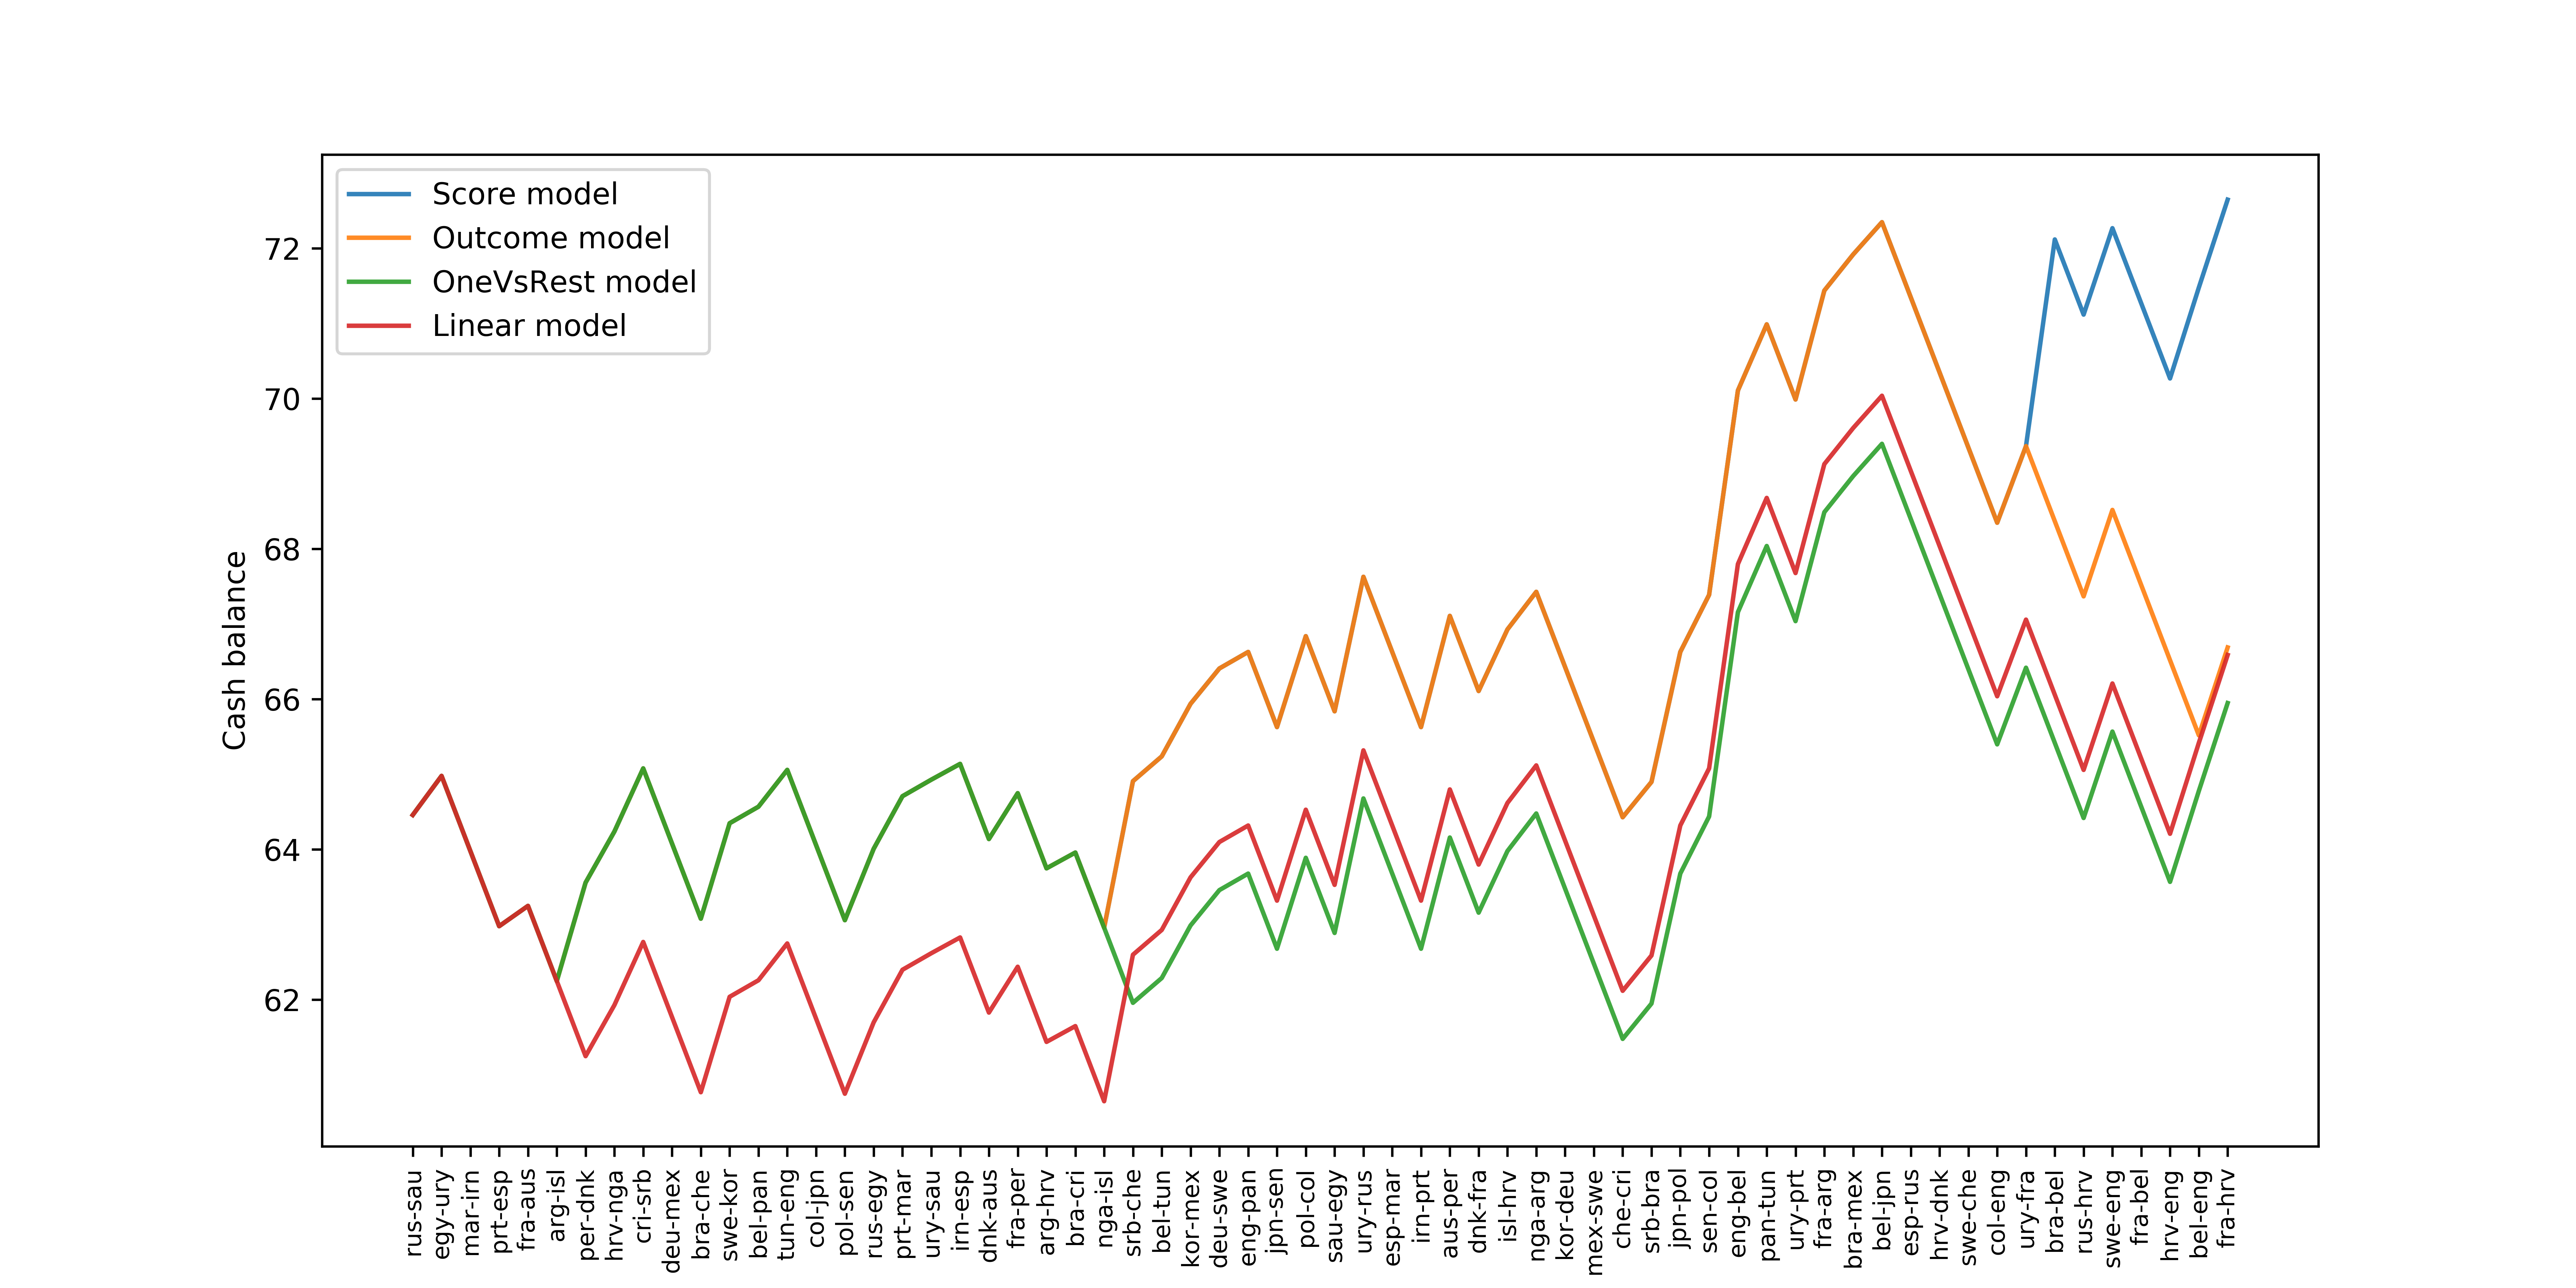
\includegraphics[width=0.7\textwidth]{img/match_level_2018_model_unit.png}
    \caption{Unit strategy's cash balance progression on World Cup 2018.}
    \label{fig:unit_model_comparison}
\end{figure}

\begin{figure}[H]
    \centering
    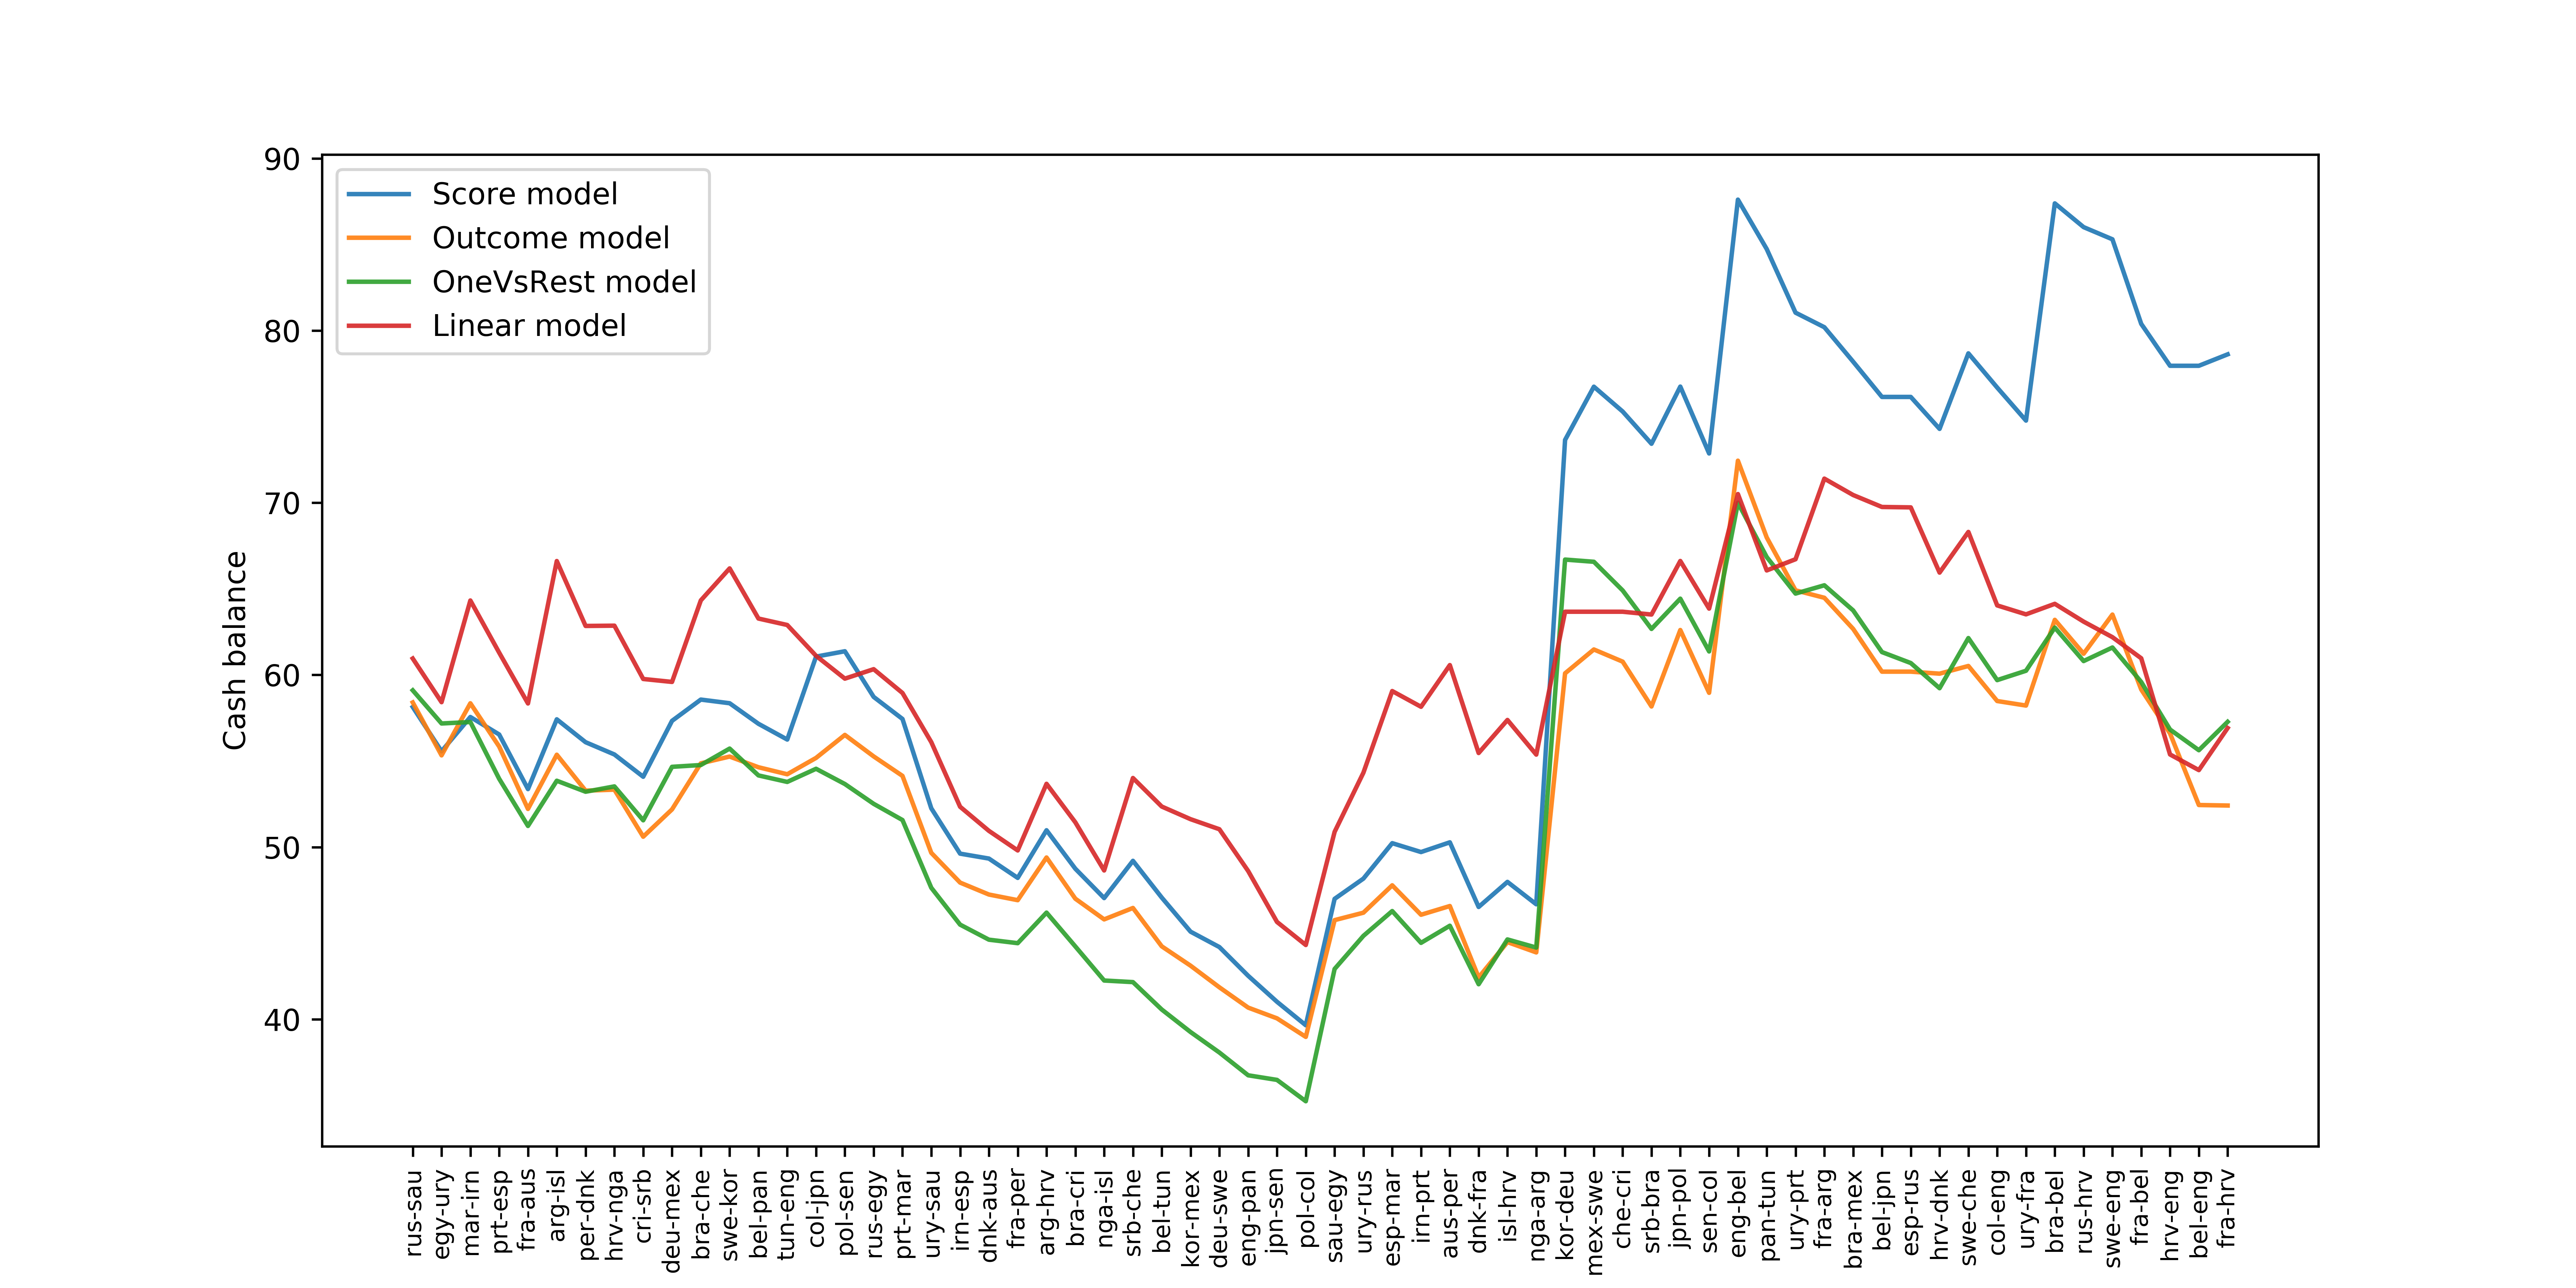
\includegraphics[width=0.7\textwidth]{img/match_level_2018_model_kelly.png}
    \caption{Kelly strategy's cash balance progression on World Cup 2018.}
    \label{fig:kelly_model_comparison}
\end{figure}

\begin{figure}[H]
    \centering
    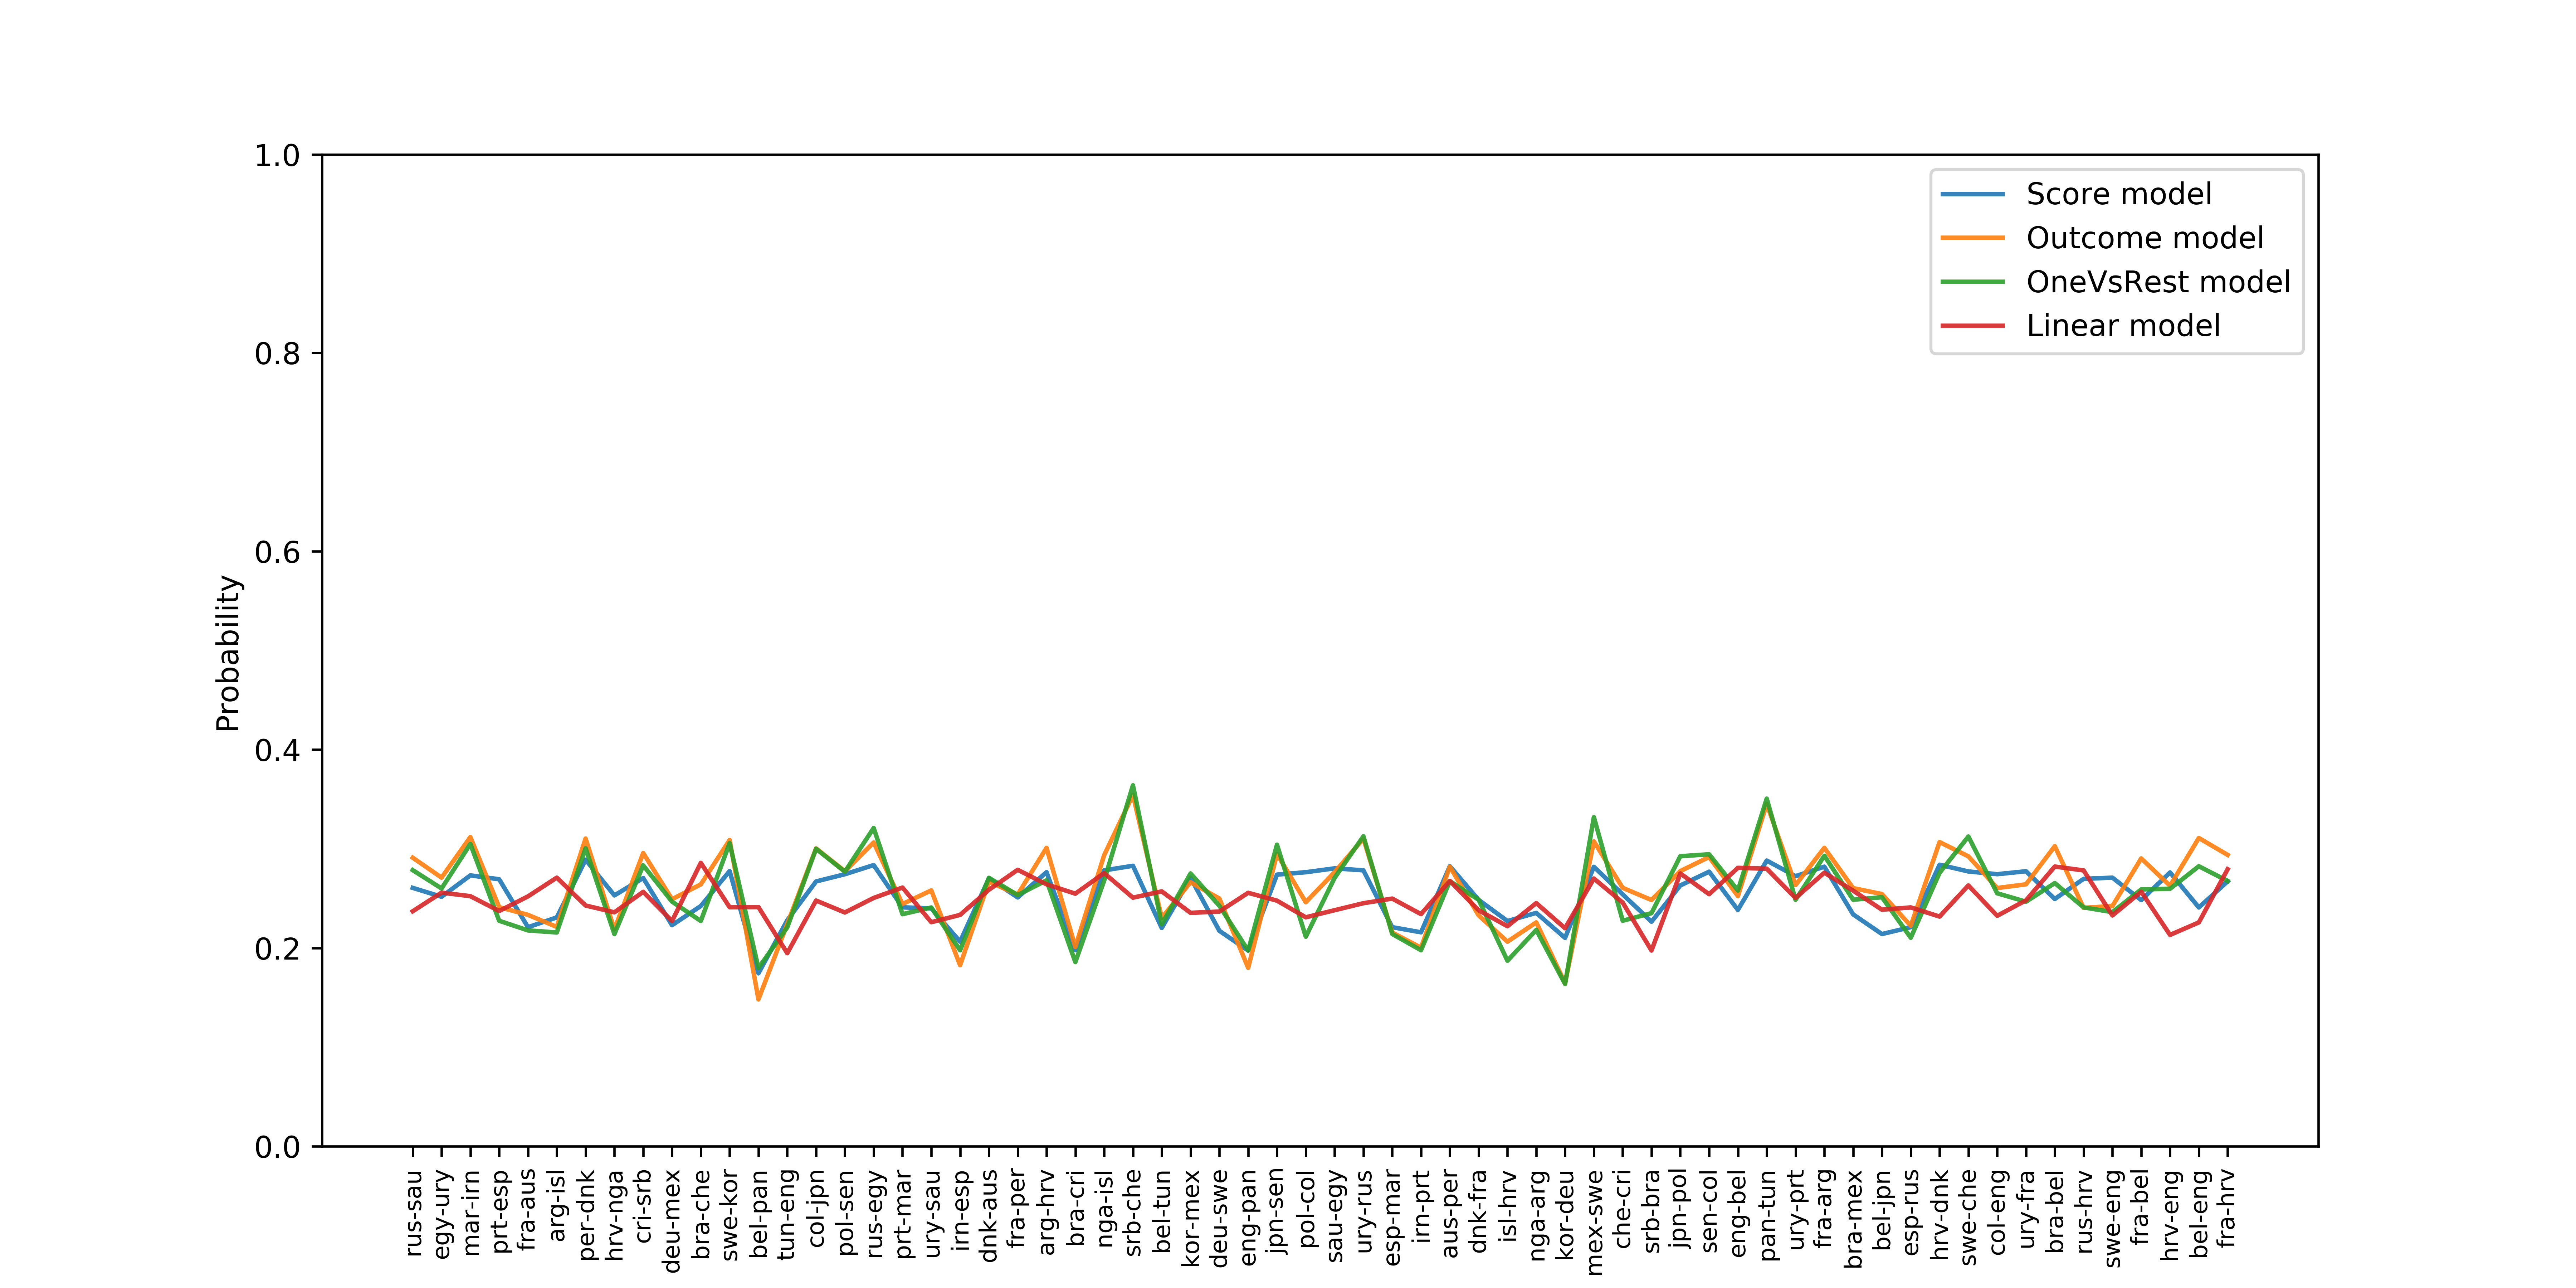
\includegraphics[width=0.7\textwidth]{img/match_level_2018_model_probability_draw_prob.png}
    \caption{Predicted probability of draw in the World Cup 2018.}
    \label{fig:draw_probability}
\end{figure}


\section{Feature set differences}
It's interesting that narrower feature sets can produce better accuracy. How can less describe more? It's against common sense, right?

These problems are visible if models' accuracy is compared. Being one of the most important metrics, it's still not the most important for the sophisticated betting strategies like kelly, which utilizes model's probability estimates. Log loss
is a metric that can be used to compare probability distributions' accuracy. A smaller value indicates a more accurate estimate. When log loss is compared per tournament model trained with limited feature set can have lower log loss value than the same model that is trained using all of the features. But when average performance from every tournament is considered training model with all features seems to output the lowest log loss score with \textit{Outcome model} and \textit{OVR model} and second lowest (only 0.0009 difference at highest) with \textit{Score model} and \textit{Linear model}. This indicates that even-though increasing accuracy might not benefit from using all features probability distribution prediction clearly benefits. Since football games often have low scores can last minute surprises change the whole game. Underdog can beat the favourite or at least square the game. This means that achieving high accuracy is hard, but fixing probabilities to match the true ones has more room to improve.

Random forest includes the information on feature importance. These values can give insight on models reasoning. This data combined with optimal hyperparameters is one way to interpret the models since inspecting every single tree in the forest would be too cumbersome. Segal \cite{segal2004machine} showed that noisy variable can lead to higher optimal value for minimum samples at leaf hyperparameter. With generic features models seem to prefer higher value for the hyperparameter minimum samples at leaf as we can see from the table \ref{table:hyperparam_results}.  Figure \ref{fig:outcome_feature_importance_gf} lists feature's importance for Outcome model trained with generic features. Difference between elo rating dominates the others, but just by looking at the plot it's impossible to say if any of the features could be considered to be just noise. Lower importance features like \textit{home\_goal} and \textit{away\_goal} seem to be in the middle tier when model is trained with all features. This higher importance compared to other features could mean that these features have predicting power. Comparing figures \ref{fig:outcome_feature_importance_af}, \ref{fig:outcome_feature_importance_gf} and \ref{fig:outcome_feature_importance_pf} only confirms that elo is very important feature and shows that some of the player attributes rank high. So it's clear what features are important but not that clear what features are unimportant - if any of them are.

\begin{table}
    \caption{Hyperparameter selection results for random forest models.}
    \begin{tabular}{| c  c| c| c| c|}
        \hline
        Model & Features & \# of predictors & Min samples at leaf & Max depth\\
        \hline
        Score & AF & $\sqrt{M}$ & 1 & 8 \\
         & GF & $\log_2{M}$ & 10 & 8 \\
         & PF & $\sqrt{M}$ & 5 & Na \\
         \hline
        Outcome & AF & $\sqrt{M}$ & 3 & 8 \\
         & GF & $\log_2{M}$ & 15 & 5 \\
         & PF & $\log_2{M}$ & 3 & 8 \\
        \hline
        OVR & AF home win & $\sqrt{M}$ & 3 & 5 \\
        OVR & AF draw & $\sqrt{M}$ & 5 & Na \\
        OVR & AF away win & $\sqrt{M}$ & 3 & 5 \\
        OVR & GF home win & $\sqrt{M}$ & 10 & 12 \\
        OVR & GF draw & $\log_2{M}$ & 15 & 8 \\
        OVR & GF away win & $\log_2{M}$ & 10 & 5 \\
        OVR & PF home win & $\log_2{M}$ & 3 & 5 \\
        OVR & PF draw & $\log_2{M}$ & 15 & 5 \\
        OVR & PF away win & $\log_2{M}$ & 5 & 8 \\
        \hline
    \end{tabular}
    \label{table:hyperparam_results}
\end{table}

\begin{figure}[H]
    \centering
    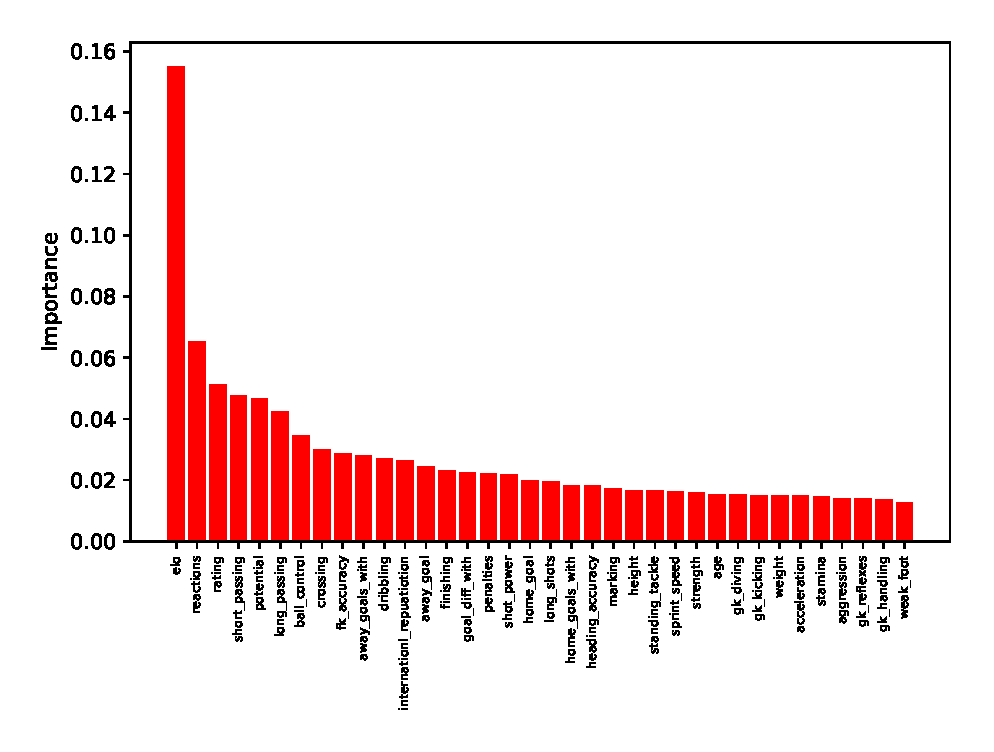
\includegraphics[width=0.7\textwidth]{img/match_level_2018_outcome_feature_importance_af_feature_importance.eps}
    \caption{Outcome model's feature importance with all features.}
    \label{fig:outcome_feature_importance_af}
\end{figure}

\begin{figure}[H]
    \centering
    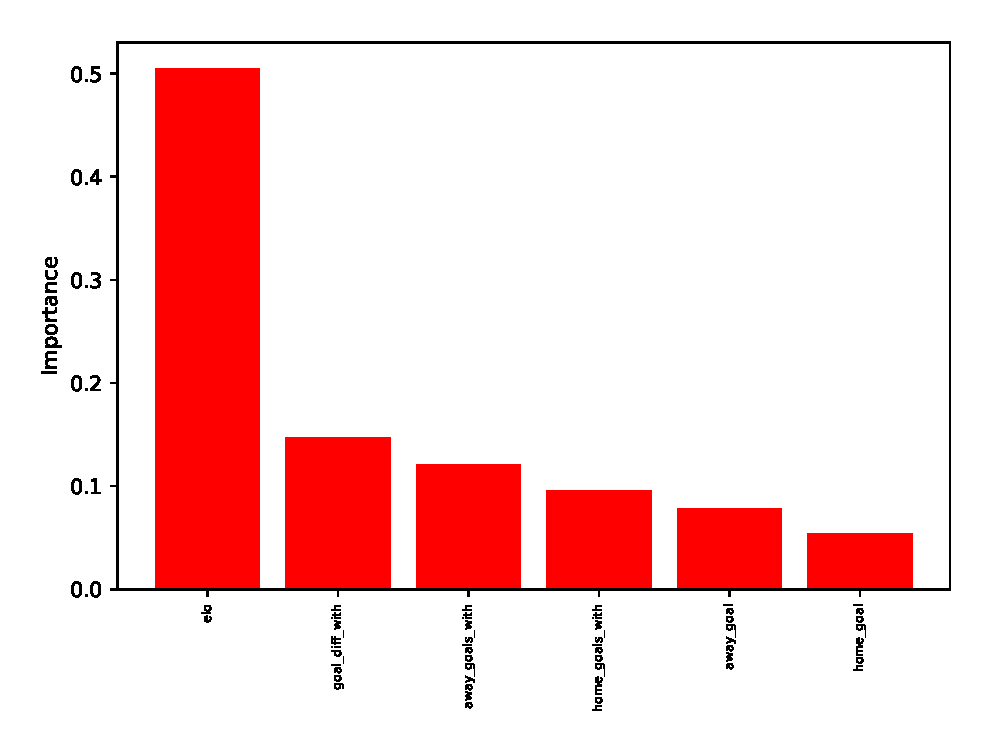
\includegraphics[width=0.7\textwidth]{img/match_level_2018_outcome_feature_importance_gf_feature_importance.eps}
    \caption{Outcome model's feature importance with generic features.}
    \label{fig:outcome_feature_importance_gf}
\end{figure}

\begin{figure}[H]
    \centering
    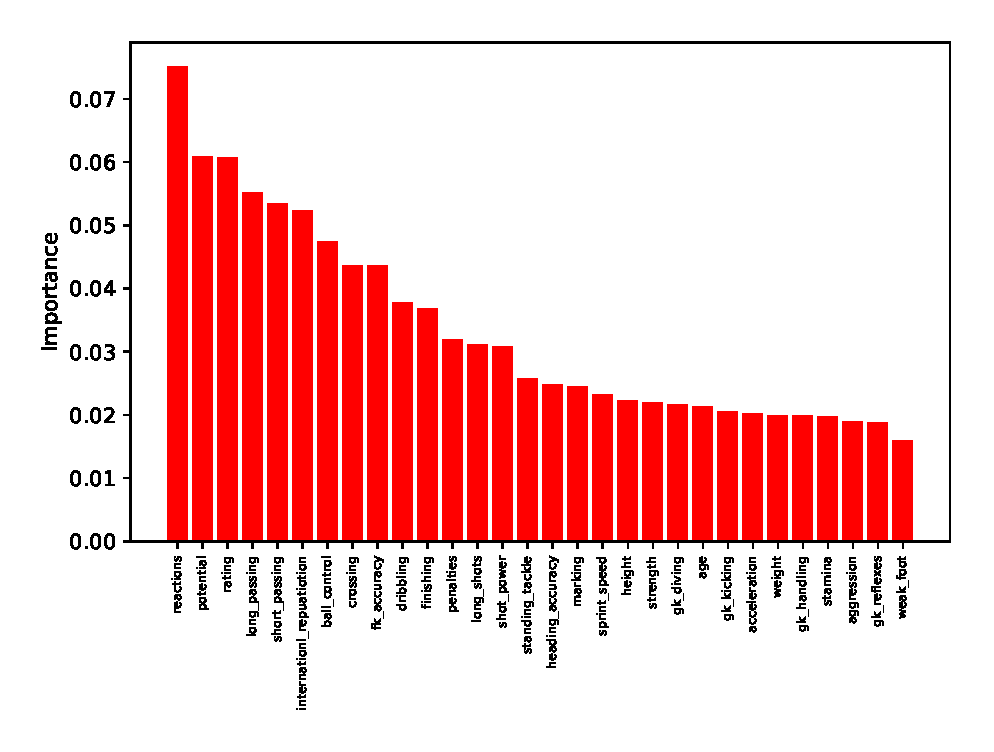
\includegraphics[width=0.7\textwidth]{img/match_level_2018_outcome_feature_importance_pf_feature_importance.eps}
    \caption{Outcome model's feature importance with player features.}
    \label{fig:outcome_feature_importance_pf}
\end{figure}


\subsection{Match-level betting activity - what drives the profits?}
\subsection{RFE for best model}
